%%%%%%%%%%%%%%%%%%%%%%%%%%%%%%%%%%%%%%%%%%%%%%%%%%%%%%%%%%%%%%%%%%%%%%
% LaTeX Template: Curriculum Vitae
%
% Source: http://www.howtotex.com/
% Feel free to distribute this template, but please keep the
% referal to HowToTeX.com.
% Date: July 2011
% 
%%%%%%%%%%%%%%%%%%%%%%%%%%%%%%%%%%%%%%%%%%%%%%%%%%%%%%%%%%%%%%%%%%%%%%
% How to use writeLaTeX: 
%
% You edit the source code here on the left, and the preview on the
% right shows you the result within a few seconds.
%
% Bookmark this page and share the URL with your co-authors. They can
% edit at the same time!
%
% You can upload figures, bibliographies, custom classes and
% styles using the files menu.
%
% If you're new to LaTeX, the wikibook is a great place to start:
% http://en.wikibooks.org/wiki/LaTeX
%
%%%%%%%%%%%%%%%%%%%%%%%%%%%%%%%%%%%%%%%%%%%%%%%%%%%%%%%%%%%%%%%%%%%%%%
\documentclass[paper=a4,fontsize=11pt]{scrartcl} % KOMA-article class
							
\usepackage[english]{babel}
\usepackage[utf8x]{inputenc}
\usepackage[protrusion=true,expansion=true]{microtype}
\usepackage{amsmath,amsfonts,amsthm}     % Math packages
\usepackage{graphicx}                    % Enable pdflatex
\usepackage[svgnames]{xcolor}            % Colors by their 'svgnames'
\usepackage{geometry}
	\textheight=700px                    % Saving trees ;-)
\usepackage{url}

\frenchspacing              % Better looking spacings after periods
\pagestyle{empty}           % No pagenumbers/headers/footers

%%% Custom sectioning (sectsty package)
%%% ------------------------------------------------------------
\usepackage{sectsty}

\sectionfont{%			            % Change font of \section command
	\usefont{OT1}{phv}{b}{n}%		% bch-b-n: CharterBT-Bold font
	\sectionrule{0pt}{0pt}{-5pt}{3pt}}

%%% Macros
%%% ------------------------------------------------------------
\newlength{\spacebox}
\settowidth{\spacebox}{8888888888}			% Box to align text
\newcommand{\sepspace}{\vspace*{9pt}}		% Vertical space macro

\newcommand{\MyName}[1]{ % Name
		\Huge \usefont{OT1}{phv}{b}{n} \hfill #1
		\par \normalsize \normalfont}
		
\newcommand{\MySlogan}[1]{ % Slogan (optional)
		\large \usefont{OT1}{phv}{m}{n}\hfill \textit{#1}
		\par \normalsize \normalfont}

\newcommand{\NewPart}[1]{\section*{\uppercase{#1}}}

\newcommand{\PersonalEntry}[2]{
		\noindent\hangindent=2em\hangafter=0 % Indentation
		\parbox{\spacebox}{        % Box to align text
		\textit{#1}}		       % Entry name (birth, address, etc.)
		\hspace{1.5em} #2 \par}    % Entry value

\newcommand{\SkillsEntry}[2]{      % Same as \PersonalEntry
		\noindent\hangindent=2em\hangafter=0 % Indentation
		\parbox{\spacebox}{        % Box to align text
		\textit{#1}}			   % Entry name (birth, address, etc.)
		\hspace{1.5em} #2 \par}    % Entry value	
		
\newcommand{\EducationEntry}[4]{
		\noindent \textbf{#1} \hfill      % Study
		\colorbox{Gray}{%
			\parbox{6.4em}{%
			\hfill\color{White}#2}} \par  % Duration
		\noindent \textit{#3} \par        % School
		\noindent\hangindent=2em\hangafter=0 \small #4 % Description
		\normalsize \par}

\newcommand{\WorkEntry}[4]{				  % Same as \EducationEntry
		\noindent \textbf{#1} \hfill      % Jobname
		\colorbox{Gray}{\color{White}#2} \par  % Duration
		\noindent \textit{#3} \par              % Company
		\noindent\hangindent=2em\hangafter=0 \small #4 % Description
		\normalsize \par}

%%% ------------------------------------------------------------
\begin{document}
% you can upload a photo and include it here...
%\begin{wrapfigure}{l}{0.5\textwidth}
%	\vspace*{-2em}
%		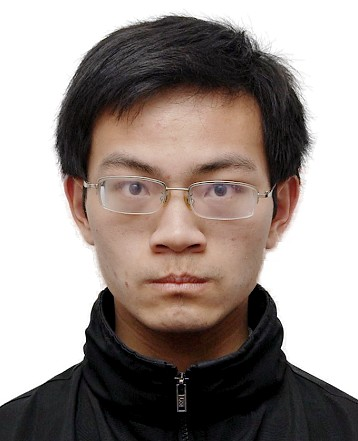
\includegraphics[width=0.15\textwidth]{photo}
%\end{wrapfigure}

\MyName{Hongxu Chen}
\MySlogan{{https://hongxuchen.github.io/}}
% \MyName{Hongxu Chen~{}~}
% \MySlogan{\url{https://hongxuchen.github.io/}}


\sepspace

%%% ------------------------------------------------------------
\NewPart{Personal details}{}

\PersonalEntry{Birth}{August 6, 1989}
\PersonalEntry{Address}{Cyber Security Lab, N4-B2C-06, NTU, Singapore}
\PersonalEntry{Phone}{+65 85476746}
\PersonalEntry{Mail}{\url{hongxuchen@outlook.com}}

%%% ------------------------------------------------------------
\NewPart{Education}{}

\EducationEntry{Ph.D in Computer Engineering}{2015.8-2019.8\\ {}~{}~{}~{}~(expected)}{Nanyang Technological University}{
I focus on Cybersecurity research in mobile applications and software. I developed a permission-dependent security type system for enforce information flow in Android, and a novel fuzzing framework by which we detected 100+ vulnerabilities in well-known open source projects.
}
\sepspace

\EducationEntry{MSc. in Computer Science}{2011.9-2014.3}{Shanghai Jiaotong University}{}
\sepspace

\EducationEntry{BSc. in Mathematics}{2007.9-2011.6}{Nanjing University of Science and Technology}{}

%%% ------------------------------------------------------------
\NewPart{Work experience}{}

\EducationEntry{Research Intern}{2013.2-2013.11}{Microsoft Research Asia, Beijing}{}
\sepspace

%%% ------------------------------------------------------------
\NewPart{Skills}{}

\SkillsEntry{Languages}{Chinese Mandarin (mother tongue), English (proficient)}
\SkillsEntry{Software}{\textsc{Rust}, \textsc{C/C++}, \textsc{Scala}, \textsc{Java}, \textsc{Python}, \textsc{Bash}, \textsc{OCaml}}
\SkillsEntry{}{Linux, Coq, Isabelle, Haskell}


%%% ------------------------------------------------------------
\NewPart{References}{}
Available on request.
% \bibliography{refs} 
% \bibliographystyle{acm}
\end{document}
